%% Local IspellDict: brasileiro
\documentclass{sciposter}
\usepackage{poster-anppom}

% usar para termos estrangeiros
\newcommand{\eng}[1]{\textit{#1}}

\title{Taxonomia de Técnicas de Visualização em Música}
\author{\textbf{Jean Menezes da Rocha, Mara Pinheiro Menezes, Marcos
    da Silva Sampaio, Natanael Ourives, Dennis Queiroz de Carvalho e
    Pedro Ribeiro Kröger Júnior}} \institute{Genos---Grupo de pesquisa
  em computação musical} \email{jean.rudess@gmail.com}

% The following commands can be used to alter the default logo settings
\leftlogo[.7]{figs/ufba-logo}{% defines logo to left of title (with scale factor)
\rightlogo[1.1]{figs/capes-logo}  % same but on right

\begin{document}

\bibliographystyle{plain}

\conference{\Large \textbf{XII Congresso da ANPPOM --- 2012
    \hfill \textsf{Grupo de Pesquisa: GENOS}}}

\maketitle

\begin{multicols}{3}

\section{Introdução}

A visualização de informações tem auxiliado para o aumento da compreensão de
dados complexos em diversas áreas como estatística, estudos sociais, e música.
A visualização de dados em música pode abranger uma gama ampla de tópicos,
trazendo consigo potenciais contribuições tanto a processos educacionais
quanto a atividades terminais de análise musical. Nosso objetivo neste trabalho
é levantar formas mais concretas e práticas de Visualização em Música. Dessa
forma decidimos propor uma taxonomia do que já tem sido implementado com tal
finalidade.

\section{Metodologia}

A classificação usada nesta taxonomia está fundamentada na proposta de Lengler e
Eppler (ver figura \ref{fig:tabela-periodica}). Sob a forma de uma tabela
periódica, ela agrupa as técnicas de visualização em grandes categorias:
Visualização de Dados, de Informação, de Conceitos, de Metáforas, de Estratégias
e Visualização Composta.

O levantamento das técnicas existente consistiu em uma coleta bibliográfica,
observação das descrições de cada técnica trabalhada e catalogação da
terminologia relevante para o tema da pesquisa. As técnicas levantadas foram
visualização em tempo real, análise harmônica, análise melódica, visualização
preditiva, visualização de coleções musicais, e finalmente ambientes integrados
de edição e visualização.

A partir da coleta de dados, procuramos inserir as informações nas categorias
adequadas da ``Tabela Periódica''.

%\subsection{Visualização em tempo real}

%\subsection{Análises harmônica e melódica}

%\subsection{Visualização preditiva}

%\subsection{Visualização de coleções musicais}

%\subsection{Ambientes integrados de edição e visualização}

\end{multicols}

\begin{multicols}{2}

\begin{figure}
  \centering
  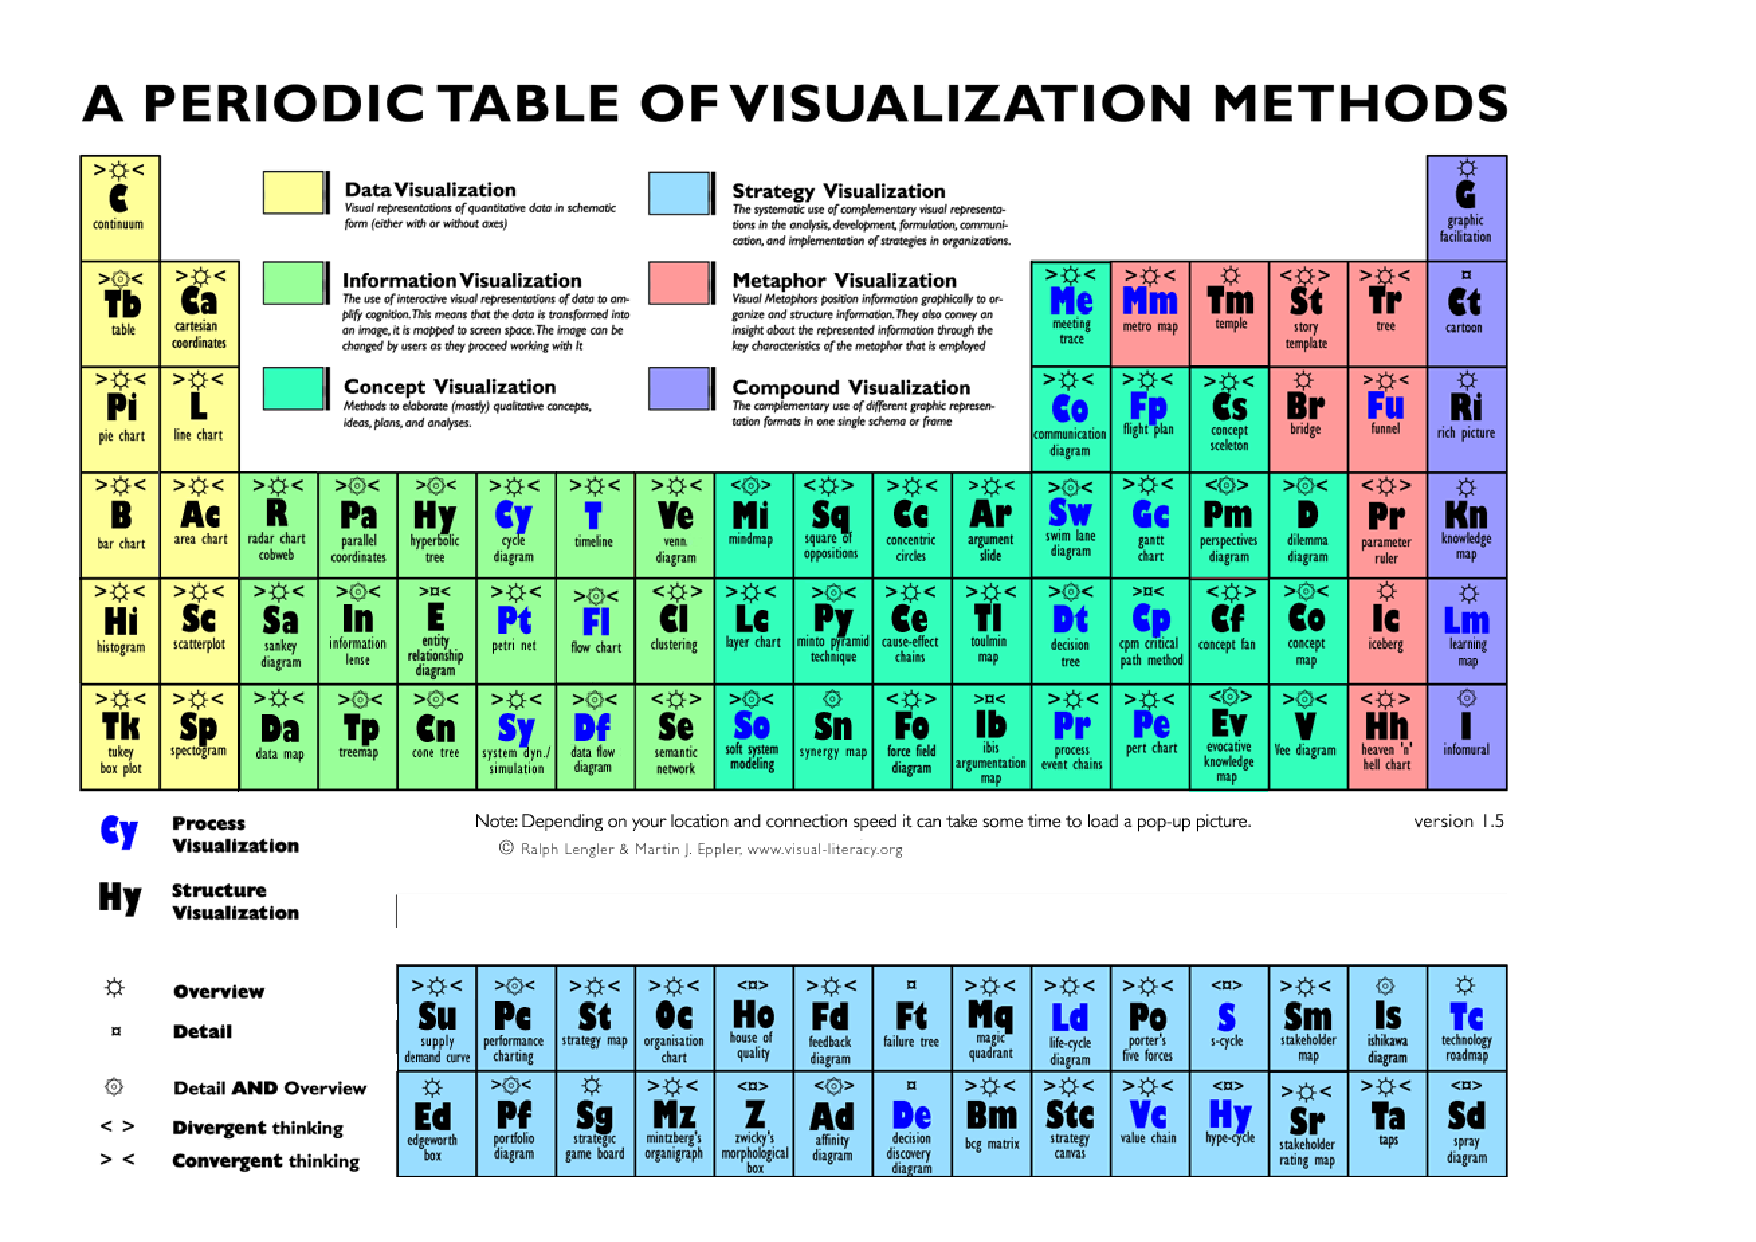
\includegraphics[scale=0.85]{tabela-periodica}
  \caption{Tabela Periódica de Métodos de Visualização \cite{Lengler2007}}
  \label{fig:tabela-periodica}
\end{figure}

\begin{figure}
  \centering
  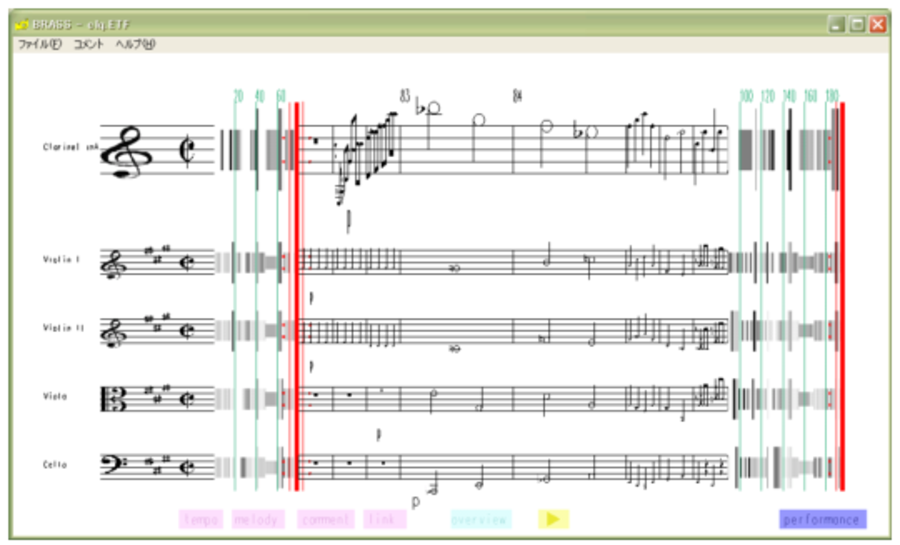
\includegraphics[scale=0.75]{watanabe-brass}
  \caption{Programa \textit{BRASS}, visualização em partitura condensada \cite{Watanabe2003}}
  \label{fig:watanabe-brass}
\end{figure}

\begin{figure}
  \centering
  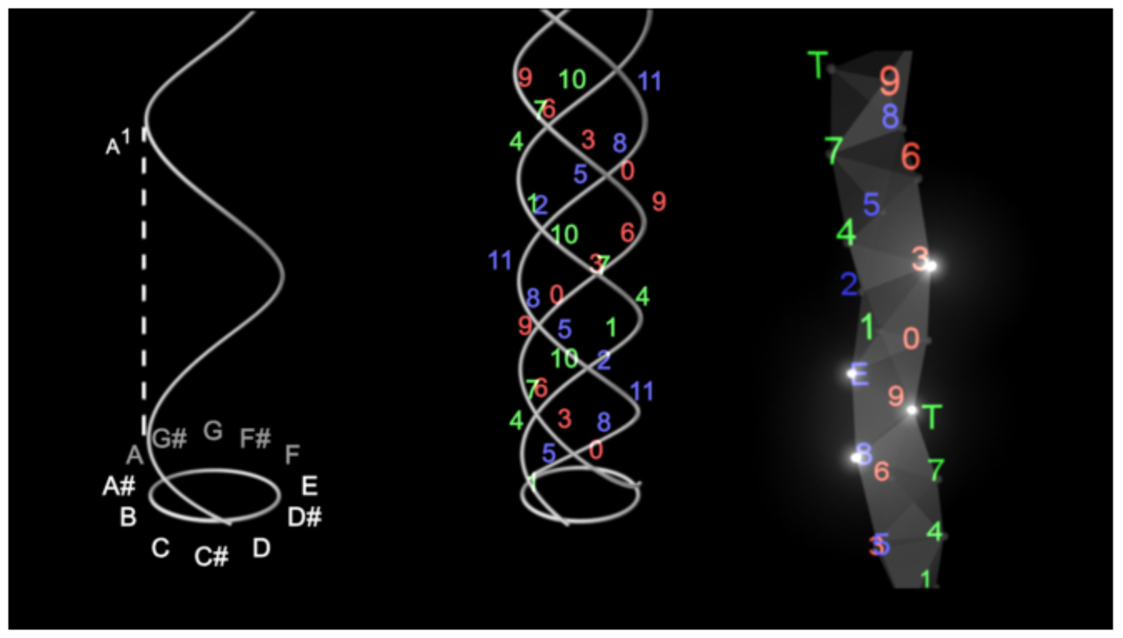
\includegraphics[scale=0.75]{bain-realtime}
  \caption{Visualização de análise harmônica automatizada \cite{Bain2008}}
  \label{fig:bain-realtime}
\end{figure}

\begin{figure}
  \centering
  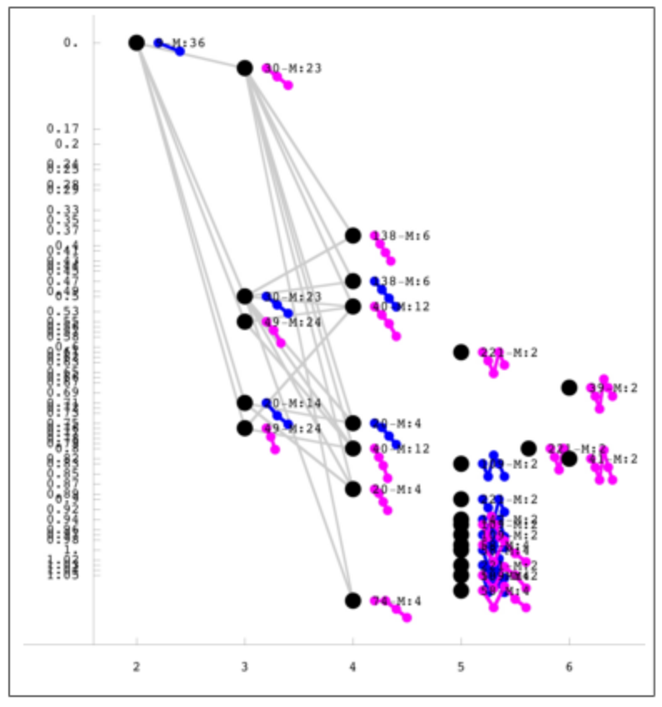
\includegraphics[scale=0.75]{buteau-motivic}
  \caption{Visualização de análise motívica automatizada \cite{Buteau2005}}
  \label{fig:buteau-motivic}
\end{figure}

\begin{figure}
  \centering
  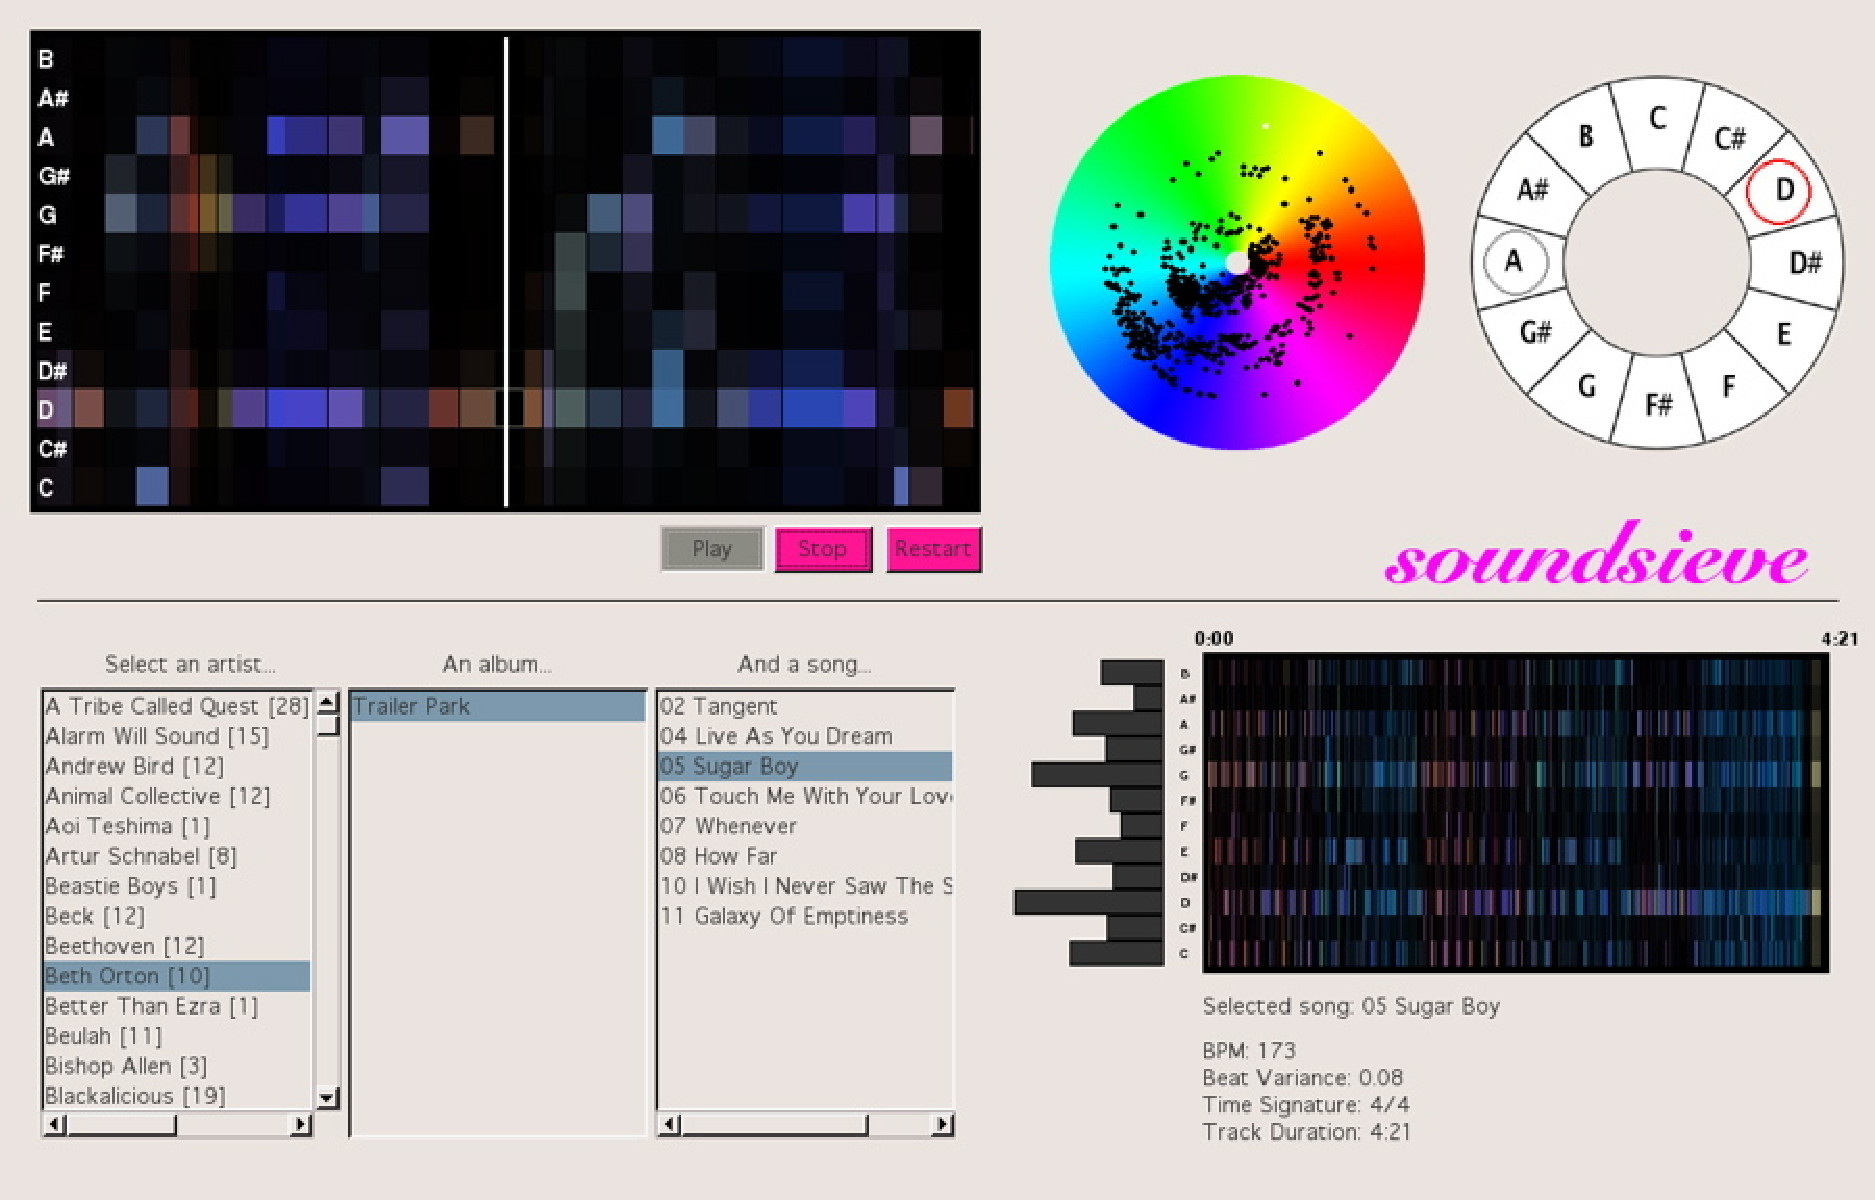
\includegraphics[scale=.7]{soundsieve}
  \caption{\textit{Soundsieve}, disponível em \url{http://bit.ly/HvL7PK}}
  \label{fig:soundsieve}
\end{figure}

\begin{figure}
  \centering
  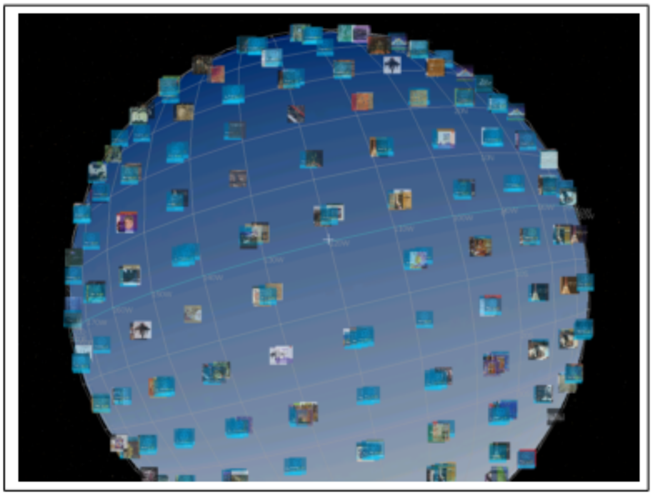
\includegraphics[scale=0.75]{topf-globe}
  \caption{Globe of Music \cite{Leitich2007}}
  \label{fig:topf-globe}
\end{figure}

\begin{figure}
  \centering
  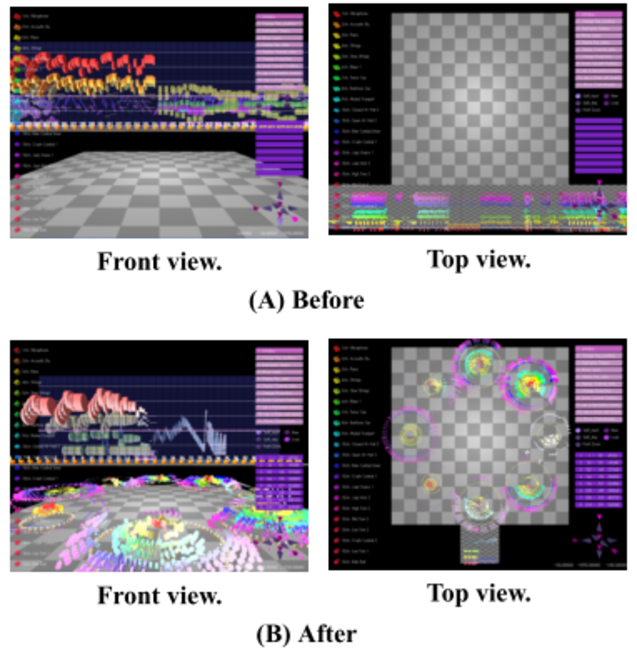
\includegraphics[scale=0.75]{comp-i}
  \caption{Programa \textit{comp-i} \cite{Miyazaki2004}}
  \label{fig:comp-i}
\end{figure}

\begin{figure}
  \centering
  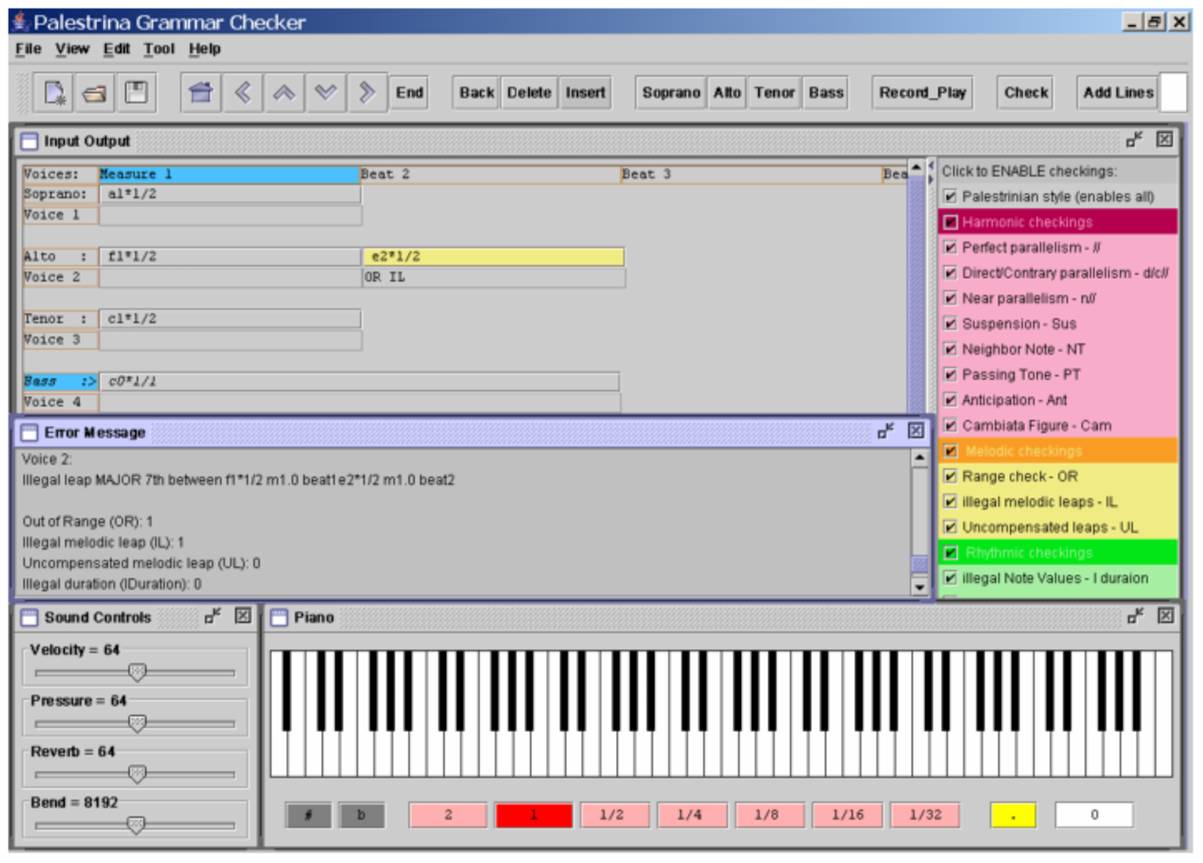
\includegraphics[scale=0.75]{palestrina-pal}
  \caption{Palestrina Pal \cite{Gramit2005}}
  \label{fig:palestrina-pal}
\end{figure}

\end{multicols}

\begin{multicols}{3}

\section{Conclusão e trabalhos futuros}

\begin{enumerate}
\item Todas as técnicas de Visualização pesquisadas possuíam ao menos uma das
propriedades associada à citada Tabela Periódica.
\item As técnicas investigadas concentram-se majoritariamente no campo de
Visualização de Informação, com um número significativo de técnicas também
situadas no campo de Visualização de Dados.
\item Os estudos de Visualização em Música estão mais focados com materiais e
instruções concretas e objetivas do que com procedimentos com maior nível de
abstração.
\item A avaliação objetiva de cada ferramenta apresentada ficou prejudicada pelo
fato de que nenhuma destas estava disponível para uso e/ou testes pelo público
em geral.
\item A Taxonomia, a princípio comparativa, é ponto de partida determinante para
a consolidação da Visualização em Música como campo de estudo.
\item Ainda é preciso verificar se a Visualização em Música deve aderir aos
princípios técnicos gerais da Visualização em caráter permanente.
\item A Visualização em Música ainda carece de técnicas para analisar
procedimentos em vez de materiais.
\end{enumerate}

\renewcommand{\refname}{Bibliografia}

\nocite{Lengler2007}

\bibliography{bibliography.bib}

\end{multicols}

\end{document}
